\documentclass[logo,reportComp]{thesis}
\usepackage[cpp,pseudo]{mypackage}

\title{分布式系统作业二}
\subtitle{}
\school{数据科学与计算机学院}
\author{陈鸿峥}
\classname{17大数据与人工智能}
\stunum{17341015}
\headercontext{分布式系统作业}

\begin{document}

\maketitle

\begin{question}
从典型的开源分布式系统如下(不限于):
\begin{itemize}
\item 分布式文件系统:HDFS、 NFS、 Ceph
\item 分布式数据库:Mongodb、 Cassandra、 ElasticSearch
\item 分布式处理框架:Hadoop、 MPI、 Spark、 Storm
\item 分布式调度器:YARN、 Mesos、 Slurm
\item 分布式操作系统:Kubernetes、 OpenStack、 OpenShift
\end{itemize}
找出分别符合集中式体系结构、非集中组织结构、混合组织结构的分布式系统,并从这些系统中选择$3\thicksim 4$个系统,找出其中能够体现分布式系统可扩展性、容错性的代码片段,并解释。
\end{question}

\section{系统分类}
其实对这些分布式系统进行分类是很难的,因为上述提及的分布式系统基本上迭代了好几年时间,当规模越做越大、业务逻辑越来越复杂时,系统设计也会产生较大变化,而且各个类别之间的界限也变得更加模糊。
因此下面的分类并不一定符合真实的情况,我只是从\textbf{官方文档}中摘录出对应的架构描述。

\subsection{集中式体系结构}
\begin{flushleft}
HDFS has a \textbf{master/slave architecture}. An HDFS cluster consists of a single NameNode, a master server that manages the file system namespace and regulates access to files by clients. In addition, there are a number of DataNodes, usually one per node in the cluster, which manage storage attached to the nodes that they run on. 
\end{flushleft}
\begin{figure}[H]
\centering
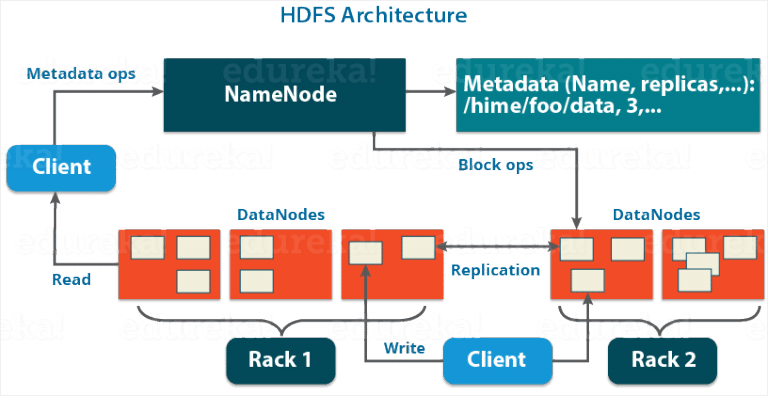
\includegraphics[width=0.8\linewidth]{fig/hdfs.png}
\caption{HDFS\cite{bib:hdfs}是分布式文件系统,采用了集中式的体系结构,单一NameNode结点,以及多个DataNodes结点。}
\end{figure}

\subsection{非集中式体系结构}
\begin{flushleft}
Ceph eliminates the centralized gateway to enable clients to interact with Ceph OSD Daemons directly. Ceph OSD Daemons create object replicas on other Ceph Nodes to ensure data safety and high availability. Ceph also uses a cluster of monitors to ensure high availability. To eliminate centralization, Ceph uses an algorithm called CRUSH. For a detailed discussion of CRUSH, see CRUSH - Controlled, Scalable, \textbf{Decentralized Placement} of Replicated Data.
\end{flushleft}
\begin{figure}[H]
\centering
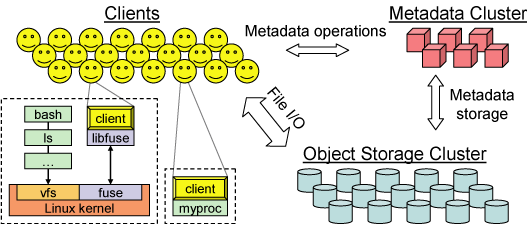
\includegraphics[width=0.8\linewidth]{fig/ceph.png}
\caption{Ceph\cite{bib:ceph}同样是分布式文件系统,但采用了去中心化的/非集中式的体系结构。}
\end{figure}

\subsection{混合体系结构}
\begin{flushleft}
Ray needs to dynamically schedule millions of tasks per second, tasks which may take as little as a few milliseconds. None of the cluster schedulers we are aware of meet these requirements.
Most cluster computing frameworks, such as Spark, CIEL, and Dryad implement a centralized scheduler, which can provide locality but at latencies in the tens of ms. Distributed schedulers such as work stealing, Sparrow and Canary can achieve high scale, but they either don’t consider data locality, or assume tasks belong to independent jobs [45], or assume the computation graph is known.
To satisfy the above requirements, we design a \textbf{two-level hierarchical scheduler} consisting of a global scheduler and per-node local schedulers.
\end{flushleft}
\begin{figure}[H]
\centering
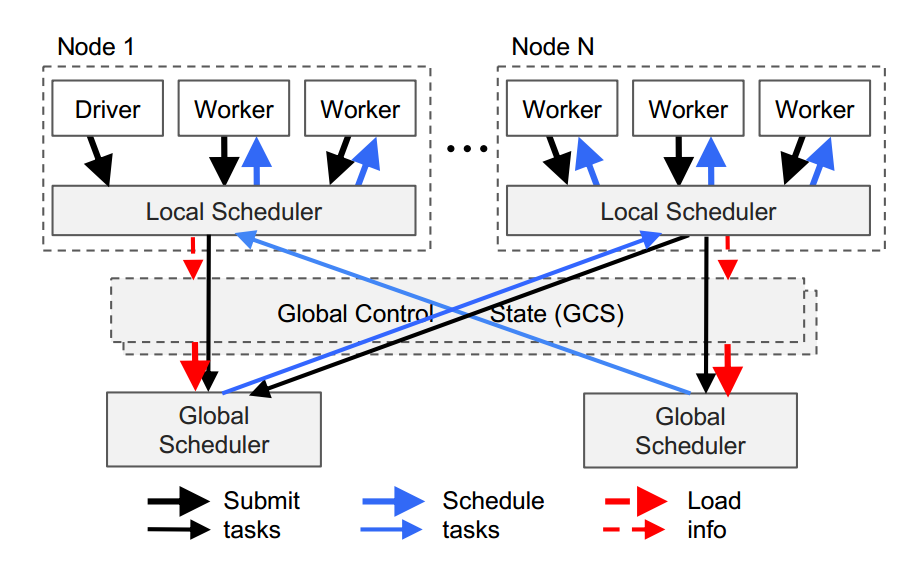
\includegraphics[width=0.8\linewidth]{fig/ray.png}
\caption{Ray\cite{bib:ray}是UCB提出来的新一代大规模机器学习系统,其调度器就采用了集中式和非集中式的两层混合架构。集中式调度器(global)有利于提取局部性信息,而非集中式调度器(local)则有利于快速部署并行。}
\end{figure}

\section{源码分析}
\subsection{可扩展性}
HDFS是可以方便地将结点扩展的,通过调用\verb'addDataNode'等一系列函数,即可将文件系统扩展到更大地集群上。
下面的添加数据结点的函数逻辑也十分简单\footnote{\url{https://github.com/apache/hadoop/blob/release-3.2.1-RC0/hadoop-hdfs-project/hadoop-hdfs/src/main/java/org/apache/hadoop/hdfs/server/blockmanagement/DatanodeManager.java\#L767}},根本原因是系统抽象做得好,并且将执行逻辑和控制逻辑进行分离。
\begin{lstlisting}[language=java]
  /** Add a datanode. */
  void addDatanode(final DatanodeDescriptor node) {
    // To keep host2DatanodeMap consistent with datanodeMap,
    // remove  from host2DatanodeMap the datanodeDescriptor removed
    // from datanodeMap before adding node to host2DatanodeMap.
    synchronized(this) {
      host2DatanodeMap.remove(datanodeMap.put(node.getDatanodeUuid(), node));
    }

    networktopology.add(node); // may throw InvalidTopologyException
    host2DatanodeMap.add(node);
    checkIfClusterIsNowMultiRack(node);
    resolveUpgradeDomain(node);

    if (LOG.isDebugEnabled()) {
      LOG.debug(getClass().getSimpleName() + ".addDatanode: "
          + "node " + node + " is added to datanodeMap.");
    }
  }
\end{lstlisting}

下面是Ray的\verb'scheduler_policy'中关于调度及添加新资源的片段\footnote{\url{https://github.com/ray-project/ray/blob/master/src/ray/raylet/scheduling_policy.cc\#L67}}。
可以看到由于分布式系统会不定时发送\verb'heartbeat',因此当有新的服务器/Worker加入时,将很容易在\verb'new_load'中通过\verb'AddResource'添加新的worker,进而实现\textbf{动态可扩展性}(调度器与底层物理架构不是紧耦合的)。
而且无论是worker数目还是集群机器数目都是参数化的(parameterizable),也方便用户将程序扩展到更大的集群上,而只需修改几个参数。
\begin{lstlisting}
    if (!client_keys.empty()) {
      // Choose index at random.
      // Initialize a uniform integer distribution over the key space.
      // TODO(atumanov): change uniform random to discrete, weighted by resource capacity.
      std::uniform_int_distribution<int> distribution(0, client_keys.size() - 1);
      int client_key_index = distribution(gen_);
      const ClientID &dst_client_id = client_keys[client_key_index];
      decision[task_id] = dst_client_id;
      // Update dst_client_id's load to keep track of remote task load until
      // the next heartbeat.
      ResourceSet new_load(cluster_resources[dst_client_id].GetLoadResources());
      new_load.AddResources(resource_demand);
      cluster_resources[dst_client_id].SetLoadResources(std::move(new_load));
    }
\end{lstlisting}

\subsection{容错性}
容错性常常采用心跳机制(heartbeat),如HDFS通过在\verb'NameNode'和\verb'DataNode'之间维持心跳检测,如果因为网络故障原因导致\verb'DataNode'发出的心跳包没有被\verb'NameNode'正常接收,则会产生异常,该\verb'DataNode'会被登记,\verb'NameNode'会自动复制新的副本给其他\verb'DataNode'。
而下面是HDFS的\verb'NameNode'中的一个函数,也采用了类似的机理,检测名字服务器是否出现资源溢出的情况\footnote{\url{https://github.com/apache/hadoop/blob/release-3.2.1-RC0/hadoop-hdfs-project/hadoop-hdfs/src/main/java/org/apache/hadoop/hdfs/server/namenode/NameNode.java\#L1769}}。
\begin{lstlisting}[language=java]
  synchronized void monitorHealth() 
      throws HealthCheckFailedException, AccessControlException {
    namesystem.checkSuperuserPrivilege();
    if (!haEnabled) {
      return; // no-op, if HA is not enabled
    }
    long start = Time.monotonicNow();
    getNamesystem().checkAvailableResources();
    long end = Time.monotonicNow();
    if (end - start >= HEALTH_MONITOR_WARN_THRESHOLD_MS) {
      // log a warning if it take >= 5 seconds.
      LOG.warn("Remote IP {} checking available resources took {}ms",
          Server.getRemoteIp(), end - start);
    }
    if (!getNamesystem().nameNodeHasResourcesAvailable()) {
      throw new HealthCheckFailedException(
          "The NameNode has no resources available");
    }
  }
\end{lstlisting}

又比如HDFS读取文件时采用的校验和\footnote{\url{https://github.com/apache/hadoop/blob/release-3.2.1-RC0/hadoop-hdfs-project/hadoop-hdfs/src/test/java/org/apache/hadoop/hdfs/server/namenode/snapshot/TestSnapshotFileLength.java\#L110}},同样是提升容错性一个重要的机制。
\begin{lstlisting}[language=java]
    final FileChecksum snapChksum1 = hdfs.getFileChecksum(file1snap1);
    assertThat("file and snapshot file checksums are not equal",
        hdfs.getFileChecksum(file1), is(snapChksum1));

    // Append to the file.
    FSDataOutputStream out = hdfs.append(file1);
    // Nothing has been appended yet. All checksums should still be equal.
    // HDFS-8150:Fetching checksum for file under construction should fail
    try {
      hdfs.getFileChecksum(file1);
      fail("getFileChecksum should fail for files "
          + "with blocks under construction");
    } catch (IOException ie) {
      assertTrue(ie.getMessage().contains(
          "Fail to get checksum, since file " + file1
              + " is under construction."));
    }
    assertThat("snapshot checksum (post-open for append) has changed",
        hdfs.getFileChecksum(file1snap1), is(snapChksum1));
    try {
      AppendTestUtil.write(out, 0, toAppend);
      // Test reading from snapshot of file that is open for append
      byte[] dataFromSnapshot = DFSTestUtil.readFileBuffer(hdfs, file1snap1);
      assertThat("Wrong data size in snapshot.",
          dataFromSnapshot.length, is(origLen));
      // Verify that checksum didn't change
      assertThat("snapshot checksum (post-append) has changed",
          hdfs.getFileChecksum(file1snap1), is(snapChksum1));
    } finally {
      out.close();
    }
    assertThat("file and snapshot file checksums (post-close) are equal",
        hdfs.getFileChecksum(file1), not(snapChksum1));
    assertThat("snapshot file checksum (post-close) has changed",
        hdfs.getFileChecksum(file1snap1), is(snapChksum1));
\end{lstlisting}

下面是Ray的\verb'Worker'中关于任务出错处理的片段\footnote{\url{https://github.com/ray-project/ray/blob/master/python/ray/worker.py\#L1002}},可以看到逻辑还是比较清晰的。
先将出错的\verb'Objects'以及中间结果全部存储起来,然后写入日志,并且将出错的\verb'actor'置为\verb'failed',最后回送出错信息。
\begin{lstlisting}[language=python]
    def _handle_process_task_failure(self, function_descriptor,
                                     return_object_ids, error, backtrace):
        function_name = function_descriptor.function_name
        failure_object = RayTaskError(function_name, backtrace)
        failure_objects = [
            failure_object for _ in range(len(return_object_ids))
        ]
        self._store_outputs_in_object_store(return_object_ids, failure_objects)
        # Log the error message.
        ray.utils.push_error_to_driver(
            self,
            ray_constants.TASK_PUSH_ERROR,
            str(failure_object),
            job_id=self.current_job_id)
        # Mark the actor init as failed
        if not self.actor_id.is_nil() and function_name == "__init__":
            self.mark_actor_init_failed(error)
        # Send signal with the error.
        ray_signal.send(ray_signal.ErrorSignal(str(failure_object)))
\end{lstlisting}

\begin{thebibliography}{99}
\bibitem{bib:hdfs} HDFS, \url{https://hadoop.apache.org/docs/r1.2.1/hdfs_design.html#Introduction}
\bibitem{bib:ceph} Ceph, \url{https://docs.ceph.com/docs/master/architecture/}
\bibitem{bib:ray} Ray, \url{https://rise.cs.berkeley.edu/projects/ray/}
\end{thebibliography}

\end{document}